\documentclass[a4paper]{article}

\setlength{\parskip}{0.1em}
\usepackage{caratula}
\usepackage[utf8]{inputenc}
\usepackage[T1]{fontenc}
\usepackage[spanish,es-tabla]{babel}
\usepackage{amsmath}
\usepackage{mathtools}
\usepackage{csquotes}
\usepackage{IEEEtrantools}
\usepackage{amssymb}
\usepackage{amsfonts}
\usepackage{fancyhdr}
\usepackage{pdfpages}
\usepackage{listings}
\usepackage{xcolor}
\usepackage{float}
\usepackage{inputenc}
\lstset { %
    language=C++,
    backgroundcolor=\color{white}, % set backgroundcolor
    basicstyle=\footnotesize,% basic font setting
}

\pagestyle{fancyplain}
% Encabezado
\lhead{Métodos Numéricos}

\begin{document}
% **************************************************************************
%
%  Package 'caratula', version 0.5.1 (para componer caratulas de TPs del DC).
%  Rev (25/02/2017): Pequeño cambio para poder usar las macros de Algo1
%  En caso de dudas, problemas o sugerencias sobre este package escribir a
%  Brian J. Cardiff (bcardif arroba gmail.com).
%  Nico Rosner (nrosner arroba dc.uba.ar).
%
% **************************************************************************

% ----- Informacion sobre el package para el sistema -----------------------

\NeedsTeXFormat{LaTeX2e}
\ProvidesPackage{caratula}[2013/08/04 v0.5 Para componer caratulas de TPs del DC]
\RequirePackage{ifthen}
\usepackage{graphicx}
\graphicspath{ {img/} }


% ----- Imprimir un mensajito al procesar un .tex que use este package -----

\typeout{Cargando package 'caratula' v0.5 (2013/08/04)}

% ----- Algunas variables --------------------------------------------------

\let\Materia\relax
\let\Submateria\relax
\let\Titulo\relax
\let\Subtitulo\relax
\let\Grupo\relax
\let\Fecha\relax
\let\Logoimagefile\relax
\newcommand{\LabelIntegrantes}{}
\newboolean{showLU}
\newboolean{showEntregas}
\newboolean{showDirectores}
\newboolean{showCoDirectores}

% ----- Comandos para que el usuario defina las variables ------------------

\def\materia#1{\def\Materia{#1}}
\def\submateria#1{\def\Submateria{#1}}
\def\titulo#1{\def\Titulo{#1}}
\def\subtitulo#1{\def\Subtitulo{#1}}
\def\grupo#1{\def\Grupo{#1}}
\def\fecha#1{\def\Fecha{#1}}
\def\logoimagefile#1{\def\Logoimagefile{#1}}

% ----- Token list para los integrantes ------------------------------------

\newtoks\intlist\intlist={}

\newtoks\intlistSinLU\intlistSinLU={}

\newcounter{integrantesCount}
\setcounter{integrantesCount}{0}
\newtoks\intTabNombre\intTabNombre={}
\newtoks\intTabLU\intTabLU={}
\newtoks\intTabEmail\intTabEmail={}

\newcounter{directoresCount}
\setcounter{directoresCount}{0}
\newtoks\direcTabNombre\direcTabNombre={}
\newtoks\direcTabEmail\direcTabEmail={}

\newcounter{coDirectoresCount}
\setcounter{coDirectoresCount}{0}
\newtoks\codirecTabNombre\codirecTabNombre={}
\newtoks\codirecTabEmail\codirecTabEmail={}


% ----- Comando para que el usuario agregue integrantes --------------------

\def\integrante#1#2#3{%
    \intlist=\expandafter{\the\intlist\rule{0pt}{1.2em}#1&#2&\tt #3\\[0.2em]}%
    \intlistSinLU=\expandafter{\the\intlistSinLU\rule{0pt}{1.2em}#1 & \tt #3\\[0.2em]}%
    %
    \ifthenelse{\value{integrantesCount} > 0}{%
        \intTabNombre=\expandafter{\the\intTabNombre & #1}%
        \intTabLU=\expandafter{\the\intTabLU & #2}%
        \intTabEmail=\expandafter{\the\intTabEmail & \tt #3}%
    }{
        \intTabNombre=\expandafter{\the\intTabNombre #1}%
        \intTabLU=\expandafter{\the\intTabLU #2}%
        \intTabEmail=\expandafter{\the\intTabEmail \tt #3}%
    }%
    \addtocounter{integrantesCount}{1}%
}

\def\director#1#2{%
    \ifthenelse{\value{directoresCount} > 0}{%
        \direcTabNombre=\expandafter{\the\direcTabNombre & #1}%
        \direcTabEmail=\expandafter{\the\direcTabEmail & \tt #2}%
    }{
        \direcTabNombre=\expandafter{\the\direcTabNombre #1}%
        \direcTabEmail=\expandafter{\the\direcTabEmail \tt #2}%
    }%
    \addtocounter{directoresCount}{1}%
}

\def\codirector#1#2{%
    \ifthenelse{\value{coDirectoresCount} > 0}{%
        \codirecTabNombre=\expandafter{\the\codirecTabNombre & #1}%
        \codirecTabEmail=\expandafter{\the\codirecTabEmail & \tt #2}%
    }{
        \codirecTabNombre=\expandafter{\the\codirecTabNombre #1}%
        \codirecTabEmail=\expandafter{\the\codirecTabEmail \tt #2}%
    }%
    \addtocounter{coDirectoresCount}{1}%
}


% ----- Macro para generar la tabla de integrantes -------------------------

\newcommand{\tablaIntegrantes}{\ }

\newcommand{\tablaIntegrantesVertical}{%
\ifthenelse{\boolean{showLU}}{%
    \begin{tabular}[t]{| l @{\hspace{4ex}} c @{\hspace{4ex}} l|}
        \hline
        \multicolumn{1}{|c}{\rule{0pt}{1.2em} \LabelIntegrantes} & LU &  \multicolumn{1}{c|}{Correo electr\'onico} \\[0.2em]
        \hline \hline
        \the\intlist
        \hline
    \end{tabular}
}{
    \begin{tabular}[t]{| l @{\hspace{4ex}} @{\hspace{4ex}} l|}
        \hline
        \multicolumn{1}{|c}{\rule{0pt}{1.2em} \LabelIntegrantes} &  \multicolumn{1}{c|}{Correo electr\'onico} \\[0.2em]
        \hline \hline
        \the\intlistSinLU
        \hline
    \end{tabular}
    }%
}

\newcommand{\tablaIntegrantesHorizontal}{%
    \begin{tabular}[t]{ *{\value{integrantesCount}}{c} }
    \the\intTabNombre \\%
\ifthenelse{\boolean{showLU}}{
    \the\intTabLU \\%
}{}
    \the\intTabEmail %
    \end{tabular}%
}

\newcommand{\tablaDirectores}{%
\ifthenelse{\boolean{showDirectores}}{%
	\bigskip
	Directores

	\smallskip
    \begin{tabular}[t]{ *{\value{directoresCount}}{c} }
    \the\direcTabNombre \\%
    \the\direcTabEmail %
    \end{tabular}%
}{}%
}

\newcommand{\tablaCoDirectores}{%
\ifthenelse{\boolean{showCoDirectores}}{%
	\bigskip
	Co-Directores

	\smallskip
    \begin{tabular}[t]{ *{\value{coDirectoresCount}}{c} }
    \the\codirecTabNombre \\%
    \the\codirecTabEmail %
    \end{tabular}%
}{}%
}

\newcommand{\tablaEntregas}{%
\ifthenelse{\boolean{showEntregas}}{%
  \bigskip%
  \begin{tabular}[t]{|l p{3.5cm} p{1.5cm}|}%
  \hline%
  \rule{0pt}{1.2em} Instancia & Docente & Nota \\[0.2em] %
  \hline%
  \hline%
  \rule{0pt}{1.2em} Primera entrega & & \\[0.2em] %
  \hline%
  \rule{0pt}{1.2em} Segunda entrega & & \\[0.2em] %
  \hline%
  \end{tabular}%
}{}%
}

% ----- Codigo para manejo de errores --------------------------------------

\def\se{\let\ifsetuperror\iftrue}
\def\ifsetuperror{%
    \let\ifsetuperror\iffalse
    \ifx\Materia\relax\se\errhelp={Te olvidaste de proveer una \materia{}.}\fi
    \ifx\Titulo\relax\se\errhelp={Te olvidaste de proveer un \titulo{}.}\fi
    \edef\mlist{\the\intlist}\ifx\mlist\empty\se%
    \errhelp={Tenes que proveer al menos un \integrante{nombre}{lu}{email}.}\fi
    \expandafter\ifsetuperror}

\def\aftermaketitle{%
  \setcounter{page}{1}
}

% ----- \maketitletxt correspondiente a la versión v0.2.1 (texto v0.2 + fecha ) ---------

\def\maketitletxt{%
    \ifsetuperror\errmessage{Faltan datos de la caratula! Ingresar 'h' para mas informacion.}\fi
    \thispagestyle{empty}
    \begin{center}
    \vspace*{\stretch{2}}
    {\LARGE\textbf{\Materia}}\\[1em]
    \ifx\Submateria\relax\else{\Large \Submateria}\\[0.5em]\fi
    \ifx\Fecha\relax\else{\Large \Fecha}\\[0.5em]\fi
    \par\vspace{\stretch{1}}
    {\large Departamento de Computaci\'on}\\[0.5em]
    {\large Facultad de Ciencias Exactas y Naturales}\\[0.5em]
    {\large Universidad de Buenos Aires}
    \par\vspace{\stretch{3}}
    {\Large \textbf{\Titulo}}\\[0.8em]
    {\Large \Subtitulo}
    \par\vspace{\stretch{3}}
    \ifx\Grupo\relax\else\textbf{\Grupo}\par\bigskip\fi
    \tablaIntegrantes
    \end{center}
    \vspace*{\stretch{3}}
    \newpage\aftermaketitle}

% ----- \maketitletxtlogo correspondiente v0.2.1 (texto con fecha y logo) ---------

\def\maketitletxtlogo{%
    \ifsetuperror\errmessage{Faltan datos de la caratula! Ingresar 'h' para mas informacion.}\fi
    \thispagestyle{empty}
    \begin{center}
    \ifx\Logoimagefile\relax\else\includegraphics{\Logoimagefile}\fi \hfill 
\includegraphics{logo_dc.jpg}\\[1em]
    \vspace*{\stretch{2}}
    {\LARGE\textbf{\Materia}}\\[1em]
    \ifx\Submateria\relax\else{\Large \Submateria}\\[0.5em]\fi
    \ifx\Fecha\relax\else{\large \Fecha}\\[0.5em]\fi
    \par\vspace{\stretch{1}}
    {\large Departamento de Computaci\'on}\\[0.5em]
    {\large Facultad de Ciencias Exactas y Naturales}\\[0.5em]
    {\large Universidad de Buenos Aires}
    \par\vspace{\stretch{3}}
    {\Large \textbf{\Titulo}}\\[0.8em]
    {\Large \Subtitulo}
    \par\vspace{\stretch{3}}
    \ifx\Grupo\relax\else\textbf{\Grupo}\par\bigskip\fi
    \tablaIntegrantes
    \end{center}
    \vspace*{\stretch{4}}
    \newpage\aftermaketitle}

% ----- \maketitlegraf correspondiente a la versión v0.3 (gráfica) -------------

\def\maketitlegraf{%
    \ifsetuperror\errmessage{Faltan datos de la caratula! Ingresar 'h' para mas informacion.}\fi
%
    \thispagestyle{empty}

    \ifx\Logoimagefile\relax\else\includegraphics{\Logoimagefile}\fi \hfill 
\includegraphics{logo_dc.jpg}

    \vspace*{.06 \textheight}

    \noindent \textbf{\huge \Titulo}  \medskip \\
    \ifx\Subtitulo\relax\else\noindent\textbf{\large \Subtitulo} \\ \fi%
    \noindent \rule{\textwidth}{1 pt}

    {\noindent\large\Fecha \hspace*\fill \Materia} \\
    \ifx\Submateria\relax\else{\noindent \hspace*\fill \Submateria}\fi%

    \medskip%
    \begin{center}
        \ifx\Grupo\relax\else\textbf{\Grupo}\par\bigskip\fi
        \tablaIntegrantes

        \tablaDirectores

        \tablaCoDirectores

        \tablaEntregas
    \end{center}%
    \vfill%
%
    \begin{minipage}[t]{\textwidth}
        \begin{minipage}[t]{.55 \textwidth}
            
\includegraphics{logo_uba.jpg}
        \end{minipage}%%
        \begin{minipage}[b]{.45 \textwidth}
            \textbf{\textsf{Facultad de Ciencias Exactas y Naturales}} \\
            \textsf{Universidad de Buenos Aires} \\
            {\scriptsize %
            Ciudad Universitaria - (Pabell\'on I/Planta Baja) \\
                Intendente G\"uiraldes 2610 - C1428EGA \\
            Ciudad Aut\'onoma de Buenos Aires - Rep. Argentina \\
                Tel/Fax: (++54 +11) 4576-3300 \\
            http://www.exactas.uba.ar \\
            }
        \end{minipage}
    \end{minipage}%
%
    \newpage\aftermaketitle}

% ----- Reemplazamos el comando \maketitle de LaTeX con el nuestro ---------
\renewcommand{\maketitle}{\maketitlegraf}

% ----- Dependiendo de las opciones ---------
%
% opciones:
%   txt     : caratula solo texto.
%   txtlogo : caratula txt con logo del DC y del grupo (opcional).
%   graf    : (default) caratula grafica con logo del DC, UBA y del grupo (opcional).
%
\@makeother\*% some package redefined it as a letter (as color.sty)
%
% Layout general de la caratula
%
\DeclareOption{txt}{\renewcommand{\maketitle}{\maketitletxt}}
\DeclareOption{txtlogo}{\renewcommand{\maketitle}{\maketitletxtlogo}}
\DeclareOption{graf}{\renewcommand{\maketitle}{\maketitlegraf}}
%
% Etiqueta Autores o Integrantes
%
\DeclareOption{integrante}{\renewcommand{\LabelIntegrantes}{Integrante}}
\DeclareOption{autor}{\renewcommand{\LabelIntegrantes}{Autor}}
%
% Formato tabla de integrantes
%
\DeclareOption{intVert}{\renewcommand{\tablaIntegrantes}{\tablaIntegrantesVertical}}
\DeclareOption{intHoriz}{\renewcommand{\tablaIntegrantes}{\tablaIntegrantesHorizontal}}
\DeclareOption{conLU}{\setboolean{showLU}{true}}
\DeclareOption{sinLU}{\setboolean{showLU}{false}}
\DeclareOption{conEntregas}{\setboolean{showEntregas}{true}}
\DeclareOption{sinEntregas}{\setboolean{showEntregas}{false}}
\DeclareOption{showDirectores}{\setboolean{showDirectores}{true}}
\DeclareOption{hideDirectores}{\setboolean{showDirectores}{false}}
\DeclareOption{showCoDirectores}{\setboolean{showCoDirectores}{true}}
\DeclareOption{hideCoDirectores}{\setboolean{showCoDirectores}{false}}
%
% Opciones predeterminadas
%
\ExecuteOptions{intVert}%
\ExecuteOptions{graf}%
\ExecuteOptions{integrante}%
\ExecuteOptions{conLU}%
\ExecuteOptions{hideDirectores}%
\ExecuteOptions{hideCoDirectores}%
\ExecuteOptions{sinEntregas}%
%
\ProcessOptions\relax

%TODO: mejorar esto cuando esté más avanzado el TP y sepamos mejor qué escribir
\begin{abstract}
    En este trabajo se busca obtener un primer acercamiento al \'area de Procesamiento del Lenguaje Natural (NLP) y al análisis de sentimiento. Además se estudia el funcionamiento y efectividad del modelo de \textit{Bag of Words} (BoW) y las técnicas algorítmicas de k vecinos más cercanos (kNN) y el análisis de componentes principales (PCA) utilizados para la identificación de emociones en reseñas de películas.


	Por medio de experimentación intentaremos obtener el mejor análisis de sentimientos posibles. La calidad de los resultados de clasificación obtenidos será analizada mediante la métrica de accuracy.
\end{abstract}

\textit{Palabras clave:} bow, knn, pca, Sentiment Analysis, NLP

\begin{figure}[H]
    \centering
    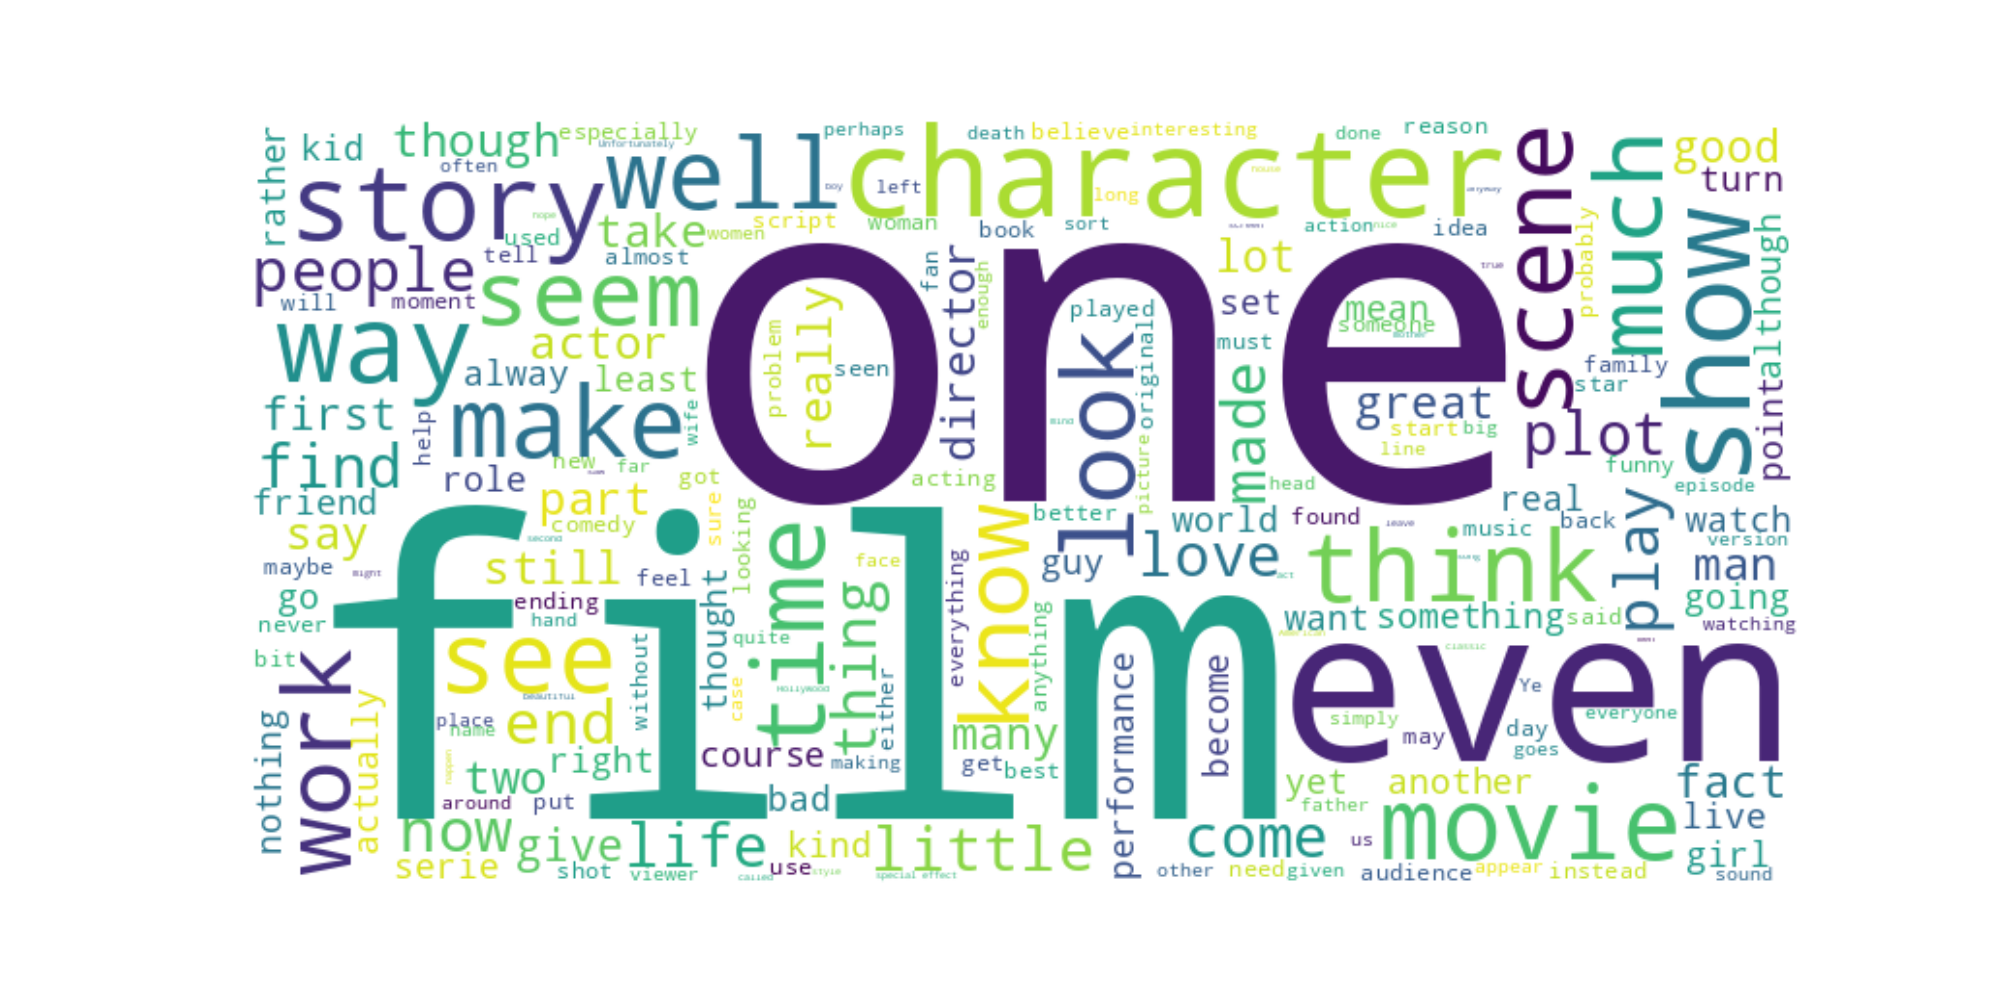
\includegraphics[ height=10cm, width=12cm]{../experimentos/wordcloud/wordcloud1.png}
    \caption{WordCloud armada con todas las palabras de las reviews}
\end{figure}


\tableofcontents

\section{Introducción}
%Contendr´a una breve explicaci´on de la base te´orica que fundamenta los m´etodos involucrados
%en el trabajo, junto con los m´etodos mismos. No deben incluirse demostraciones
%de propiedades ni teoremas, ejemplos innecesarios, ni definiciones elementales (como
%por ejemplo la de matriz sim´etrica). En vez de definiciones b´asicas es conveniente citar
%ejemplos de bibliograf´ıa adecuada. Una cita vale m´as que mil palabras.

Cada vez resulta de mayor interés el estudio de la enorme cantidad de datos
generada y distribuida por Internet. Esta puede contestar preguntas que
resultan de utilidad para múltiples usos, tanto comerciales como académicos.

A partir de estos intereses surgieron distintas técnicas con este
objetivo. Llamamos Análisis de Sentimiento, o minería de opinión, al uso de
distintas herramientas estadísticas, computacionales y lingüísticas,
con el fin de extraer información de ciertos datos, sobre la emoción, opinión o
interés de un grupo humano sobre un tema particular.

En el presente trabajo, nos proponemos utilizar algunas de estas herramientas
en el contexto particular del estudio de polaridad de reseñas de películas
en IMDb\cite{IMDB}, es decir, para clasificar estas reseñas en ``Positivas'' o ``Negativas''.

En particular, utilizaremos:
\begin{itemize}
    \item Modelo de Bag of Words
    \item Análisis de Componentes Principales (PCA)
    \item Clasificación mediante k vecinos más cercanos (kNN)
\end{itemize}
Las mismas serán explicadas más detalladamente en la siguiente sección.

Tenemos como objetivo estudiar la efectividad de las herramientas utilizadas,
experimentando con la variación de distintos hiperparámetros y de la cantidad de datos
suministrados, teniendo en cuenta el tiempo de cómputo tomado.
Este último punto resulta importante dado que uno no puede esperar indefinidamente
los resultados de un experimento, pero además es crucial si se desea
utilizar en un sistema en tiempo real como, por ejemplo, una web que recomiende películas.



%Poder extraer informaci\'on de lo que mencionan los usuarios en Internet es un tema que est\'a muy de moda hace ya unos cuantos años y que ha tenido su boom con la eclosi\'on de las Redes Sociales\cite{BO}. Un uso potencial de estas opiniones se encuentra en lo comercial: ¿Qu\'e opinan los televidentes de la nueva serie original de Netflix? ¿Hablan en Twitter positivamente de la nueva camiseta de Boca Juniors? ¿Gust\'o la nueva pel\'icula de Marvel?
%Los intereses sobre este campo trascienden lo comercial, por ejemplo la posibilidad de analizar cuantitativamente las opiniones de los usuarios (y votantes) despierta intereses pol\'iticos: ¿Qu\'e candidato tiene la mejor opini\'on de los votantes? ¿A qu\'e referente pol\'itico critican m\'as en las redes sociales? Son preguntas que atacan muchas consultoras.\\

%El Análisis de sentimiento (también conocido como minería de opinión) se refiere al uso de procesamiento del lenguaje natural (NLP), análisis de texto y lingüística computacional para identificar y extraer información subjetiva de los recursos. Desde el punto de vista de la minería de textos, el análisis de sentimientos es una tarea de clasificación masiva de documentos de manera automática, en función de la connotación positiva o negativa del lenguaje ocupado en el documento.\cite{LIU} Es importante mencionar que estos tratamientos generalmente "se basan en relaciones estadísticas y de asociación, no en análisis lingüístico".\cite{Weiss} \\
%En términos generales, el análisis de sentimiento intenta determinar la actitud de un interlocutor o usuario con respecto a algún tema o la polaridad contextual general de un documento. La actitud puede ser su juicio o evaluación, estado afectivo (o sea, el estado emocional del autor al momento de escribir), o la intención comunicativa emocional (o sea, el efecto emocional que el autor intenta causar en el lector). \\

%Una tarea básica en análisis de sentimientos es clasificar la polaridad de un texto dado, siendo esta la motivaci\'on del presente trabajo. En el mismo construiremos un analizador de polaridad para las opiniones sobre pel\'iculas de usuarios de IMDB \cite{IMDB}. Para ello, construiremos un clasificador basado en la t\'ecnica de vecinos m\'as cercanos (K-Nearest Neighbors) y reducci\'on de la dimensionalidad con an\'alisis de componentes principales (Principal Component Analysis). Posteriormente, probaremos mediante experimentaci\'on las t\'ecnicas y metedolog\'ias utilizadas, logrando así una primera noci\'on y un primer acercamiento al análisis de sentimiento y sus problem\'aticas.

\section{Desarrollo}
%Deben explicarse los m´etodos num´ericos que utilizaron y su aplicaci´on al problema
%concreto involucrado en el trabajo pr´actico. Se deben mencionar los pasos que siguieron
%para implementar los algoritmos, las dificultades que fueron encontrando y la
%descripci´on de c´omo las fueron resolviendo. Explicar tambi´en c´omo fueron planteadas
%y realizadas las mediciones experimentales. Los ensayos fallidos, hip´otesis y conjeturas
%equivocadas, experimentos y m´etodos malogrados deben figurar en esta secci´on, con
%una breve explicaci´on de los motivos de estas fallas (en caso de ser conocidas).

\subsection{Dataset de Reseñas}
%El conjunto de datos a utilizar está basado en el Large Movie Review Dataset el cual fue creado para el trabajo de Maas et al.\cite{Maas}. Consta de 50.000 reseñas de películas de obtenidas de IMDB, segmentadas en positivas (aquellas que tuvieron puntaje mayor a 7 estrellas) y negativas (puntaje menor a 4).
%El dataset está partido exactamente en dos: 25.000 instancias de entrenamiento, y otras 25.000 instancias de testeo. A su vez, las instancias de entrenamiento y testing tienen la mitad de reseñas positivas, y la otra mitad negativas.

Para poder testear las herramientas que utilizaremos para el Análisis de Sentimiento,
y poder detectar la polaridad dado el texto de una reseña de una película,
es decir, si esta es negativa o positiva, utilizaremos un
dataset de 50.000 reseñas de películas obtenidas de IMDb.
Este está basado en el \textit{Large Movie Review Dataset},
creado por Maas et al.\cite{Maas}.
Se encuentran clasificadas en \textit{positivas}
(aquellas que tuvieron puntaje mayor a 7 estrellas, siendo 25.000 instancias)
y \textit{negativas}(puntaje menor a 4, obteniendo otras 25.000 instancias),
de las cuales la mitad de las instancias son de entrenamiento y la otra mitad de testing.


\subsection{Metodología}
%Como algoritmo de clasificación utilizaremos k vecinos más cercanos (kNN, k-Nearest Neighbors). En su versión más simple, este algoritmo considera a cada instancia de entrenamiento (en nuestro caso, cada reseña) como un punto en el espacio euclídeo m-dimensional. Cuando queramos clasificar una instancia como positiva o negativa, buscaremos las k instancias de entrenamiento más cercanas y le daremos la etiqueta mayoritaria entre esos vecinos.\\

Para la clasificación según la polaridad(\textit{positiva} o \textit{negativa})
utilizaremos el algoritmo de kNN.
Para ello, este algoritmo considera a cada instancia como un punto en un plano euclídeo
(el método es descrito en más detalle en la sección \ref{sec:knn}).

%La entrada de kNN deben ser vectores de $\mathbb{R}^{m}$, para un \textit{m} fijo, uno por cada instancia. Para convertir cada reseña en un vector de longitud fija utilizamos el modelo de Bolsa de Palabras (\textit{Bag of Words o BoW}). Dado un vocabulario precalculado (y ordenado) de palabras, ignoramos el orden de las palabras en un texto y sólo contamos cuántas veces apareció en  éste. Luego, en la coordenada \textit{i}-ésima tendremos cuántas veces apareció la palabra número \textit{i} en ese texto.\\

Para poder expresar a cada reseña como un vector de \textit{n} coordenadas,
para un \textit{n} fijo, y poder usar  el algoritmo de kNN,
utilizaremos el modelo de Bolsa de Palabras (\textit{Bag of Words o BoW}).
Este es un método que se utiliza en el procesado del lenguaje para representar
documentos ignorando el orden de las palabras. Para ello se cuenta cuantas veces aparece
cada palabra en una reseña, basándose en un diccionario con todas las palabras utilizadas.
De esta forma, obtenemos un vector de la misma
dimensión del tamaño del vocabulario que representa esta información.

El problema que presenta este modelo a simple vista es que si tenemos
un diccionario demasiado grande, generaremos vectores de igual dimensión para cada reseña.
En nuestro caso, el diccionario es de aproximadamente 160.000 palabras.
Para tratar de eludir este problema, experimentaremos filtrando
dos tipos de palabras con distintos umbrales y veremos cuál da mejores resultados:
\begin{itemize}
	\item \textbf{Aquellas con frecuencia alta:} casi siempre preposiciones, conjugaciones de verbos comunes.
	\item \textbf{Palabras con muy baja frecuencia:} no aportan información significativa para la mayoría de estos problemas, y no nos permiten encontrar un patrón común entre las diferentes clases a separar
\end{itemize}

El procedimiento de \textit{tokenización} y construcción de vectores
con \textit{Bag of Words} fue programado y entregado por la cátedra.
Por eso, sólo analizaremos los umbrales y luego nos enfocaremos en el resto de las herramientas numéricas.

También nos resulta interesante experimentar con el tamaño del dataset
de entrenamiento y los hiperparámetros de los métodos numéricos empleados.
Tendremos en cuenta al analizar el constante \textit{trade-off} entre la exactitud y tiempo de ejecución de la clasificación.

\subsubsection{K vecinos más cercanos}
\label{sec:knn}
Para clasificar las reseñas, vamos a utilizar el método de los k vecinos más cercanos (kNN).
Dada una reseña a clasificar, modelada como vector (como explicamos anteriormente),
el método consta de buscar las k reseñas del dataset de \textit{training} que
resultan más cercanas.
En particular, utilizaremos la \textit{Norma Manhattan} para medir distancias,
ya que nos interesa medir la cantidad de \textit{tokens} que \textbf{no} tienen en común.

Luego, vemos la moda de estas k reseñas y la usamos para clasificar la nuestra.
Es decir, si la mayoría de estas k reseñas son positivas, clasificaremos a la
reseña como positiva. Caso contrario, como negativa.
Utilizamos siempre valores impares de k, evitando empates que requerirían un
criterio arbitrario de desempate.

% El procedimiento puede ser resumido en los siguientes pasos:
% \begin{itemize}
% 	\item Se define una base de datos de entrenamiento como el conjunto $ D = \lbrace x_{i} : i = 1,...,n\rbrace.$
% 	\item Luego, se define m como el número total de dimensiones de la \textit{i}-ésima instancia almacenada por filas y representada como un vector $x_{i} \in \mathbb{R}^{m}$.
% 	\item De esta forma, dada una instancia $x \in \mathbb{R}^{m}$, talque $x \not\in D$, para clasificarla simplemente se busca el subconjunto de los \textit{k} vectores $\lbrace x_{i}\rbrace \subseteq D$ más cercanos a $x$, y se le asigna la clase que posea el mayor número de repeticiones dentro de ese subconjunto, es decir, la moda.
% \end{itemize}

Este algoritmo depende fuertemente del tamaño de nuestros vectores, ya que
para calcular la distancia entre dos reseñas necesitamos recorrer ambos.
Es por eso que surge la idea de reducir las dimensiones, intentando quedarse
con la información más relevante. Para eso, se considera el
\textbf{Análisis de Componentes Principales} (PCA), el cual describiremos a continuación.

% El algoritmo de los vecinos más cercanos es muy sensible a la dimensión de los objetos y a la variación de las componentes del vector instancia. Es por eso, que las instancias dentro de la base de datos se suelen preprocesar para lidiar con estos problemas.
% Teniendo en cuenta esto, una alternativa interesante de preprocesamiento es buscar reducir la cantidad de dimensiones de las muestras para trabajar con una cantidad de variables más acotada buscando que las nuevas variables tengan información representativa para clasificar los objetos de la base de entrada.
% En esta dirección, consideraremos el método de reducción de dimensionalidad Análisis de Componentes Principales o PCA (por su sigla en inglés) dejando de lado los procesamientos de datos que se puedan realizar previamente o alternativamente a aplicar PCA.

\subsubsection{Análisis de Componentes Principales}
\label{sec:pca}
El Método de Análisis de Componentes Principales se basa en la idea de que,
dado un conjunto de datos en forma de vectores (como puede ser nuestro \textit{BoW}),
hay dimensiones o \textit{componentes} que dan mayor información que otras.
Por eso, resulta interesante quedarse solo con estas componentes,
eliminando las demás, que pueden resultar redundantes o incluso meter ruido.
De esta forma se logra agilizar los cómputos posteriores y quizá incluso mejorar los resultados obtenidos,
trabajando con un vector de menor tamaño pero con información relevante y menos ruido.

Para realizar este procesamientos, utilizamos la \textbf{Matriz de Covarianza}.
Recordemos que la covarianza nos dice en qué medida dos variables
(en nuestro caso, los \textit{tokens}) varían de forma similar.
A partir de esta matriz, podemos calcular las componentes principales
quedándonos con los $\alpha$ autovectores asociados a los autovalores
de mayor valor absoluto
\footnote{Pueden verse más detalles sobre los cálculos relacionados en
http://www.cs.otago.ac.nz/cosc453/student\_tutorials/principal\_components.pdf}.

Con estos autovectores, definimos la \textit{transformación característica},
con la matriz formada por ellos puestos como fila.
De esta forma, dicha transformación toma vectores en $\mathbb{R}^{n}$ y devuelve
vectores en $\mathbb{R}^{\alpha}$, disminuyendo dimensiones pero de forma que
la información ``más relevante'' no se pierda.

El valor del hiperparámetro $\alpha$ nos da la oportunidad de experimentar,
buscando el que mejor funcione para nuestro contexto, y para ver su relación
con otros hiperparámetros.

% El método de análisis de componentes principales o PCA consiste en lo siguiente.
% Sea $ \mu = (x_{1} + . . . + x_{n})/n$ el promedio coordenada a coordenada de los datos $D = \lbrace x_{i}: i = 1,...,n\rbrace$ tal que $x_{i} \in \mathbb{R}^{m}$. Definimos $X \in \mathbb{R}^{nxm}$ como la matriz que contiene en la i-ésima fila al vector $(x_{i} - \mu)^{t}/\sqrt{n - 1}$. La matriz de covarianza de la muestra $X$ se define como $M = X^{t}X$.
%
% Siendo $v_{j}$ el autovector de $M$ asociado al \textit{j}-ésimo autovalor, al ser ordenados por su valor absoluto, definimos para $i = 1,...,n$ la \textit{transformación característica} de $x_{i}$ como el vector $\textbf{tc}(x_{i}) = (v_{1}x_{i},v_{2}x_{i},...,v_{\alpha}x_{i})^{t} \in \mathbb{R}^{\alpha}$, donde $\alpha \in \lbrace 1,...,m\rbrace$ es un parámetro de la implementación. Este proceso corresponde a extraer las $\alpha$ primeras componentes principales de cada muestra. La idea es que $\textbf{tc}(x_{i})$ resuma la información más relevante de la muestra, descartando los dimensiones menos significativas.
%
% El método PCA previamente presentado sirve para realizar una transformación de los datos de entrada a otra base y así trabajar en otro espacio con mejores propiedades que el original.

\subsubsection{Cálculo de autovectores}
Como se mencionó en la sección anterior, el método PCA utiliza los autovectores de la matriz de covarianza.
Para obtenerlos, utilizamos el Método de la Potencia\cite{pot}.

Siendo este un método iterativo, resulta de interés experimentar con el criterio de terminación.
Dado que cortamos el algoritmo luego de una cantidad determinada de iteraciones,
decidimos ver como afecta este número a la exactitud del resultado.

\subsubsection{Procedimiento para la clasificación con kNN y PCA}
Una vez elegidos los hiperparámetros, el proceso de clasificación de una reseña
nueva consta de su tokenización y pasaje al modelo de \textit{Bag of Words},
el cálculo de su transformación característica (en caso de usar PCA),
la búsqueda de los vecinos más cercanos del dataset de \textit{training}
(de acuerdo con la \textit{Norma Manhattan}) y finalmente,
la clasificación de acuerdo a la moda en estos vecinos.

Previamente, en caso de usar PCA, es necesario realizar el cálculo de las
componentes principales sobre el dataset de \textit{training},
como fue explicado en la sección \ref{sec:pca}.


%Una vez elegidos los parámetros $k$ del $kNN$ y $\alpha$ de PCA, el proceso completo de clasificación de reseñas se puede resumir como:
% \begin{enumerate}
% 	\item Ingresa una nueva reseña $x$ no presente en el conjunto de entrenamiento.
% 	\item Se computa el $x_{b} = BoW (x)$
% 	\item Se calcula $\textbf{tc}(x_{b})$ la transformación característica
% 	\item Se compara con cada $\textbf{tc}(x_{bi})$, $\forall x_{bi} \in Db$ donde $D_{b}$ es el dataset de training procesado con $BoW$
% 	\item Se elige la moda entre los $k$ vecinos más cercanos
% 	\item Se devuelve la clase de la moda (“pos” o “neg”) como el resultado de la clasificación.
% \end{enumerate}

\subsection{Programación}
Pasamos a contar las decisiones más significativas que tomamos a la hora de implementar los métodos en C++. Para más detalles, ver el código de los mismos en los apéndices o  el código fuente entregado junto a este informe.

\subsubsection{Estructuras elegidas}
Para representar las reseñas, utilizamos \textit{vector<double>} de la STL, dada su simplicidad y buen uso de la memoria caché y para las matrices utilizamos \textit{vector<vector<double>\null>}.

También vale la pena destacar que para buscar los k vecinos más cercanos, guardamos las distancias en un vector, para luego poder construir un \textit{MinHeap}. A partir de este, podemos conseguir el mejor vecino y quitarlo del \textit{MinHeap} en $O(lg(n))$. Este método resulta mejor a ordenar el vector de distancias en términos de complejidad, dado que conseguir los k vecinos más cercanos toma, sin contar el cálculo de distancias, $O(k \cdot lg(n))$, contra un $O(n \cdot lg(n))$ del ordenamiento.

\subsubsection{Optimizaciones}
Dada la lentitud en la ejecución de los experimentos decidimos buscar alternativas. El mayor problema lo teníamos principalmente en la construcción de la matriz de covarianza necesaria para PCA,  por eso decidimos realizar cálculos en paralelo utilizando \textit{threads} para calcularla. Además, agregamos una opción a nuestro ejecutable para que utilice la matriz de covarianza y autovectores calculados en alguna ejecución anterior de existir.


\subsection{Proceso de experimentación}
Luego de terminado el desarrollo del programa principal,
decidimos realizar los siguientes experimentos:

\begin{itemize}
	\item Calidad de los resultados al variar:
	\begin{itemize}
		\item El parámetro k de kNN, sin usar PCA
		\item La frecuencia mínima y máxima de palabras filtradas, sin usar PCA
		\item El tamaño del \textit{dataset} de training, con y sin PCA
		\item El parámetro alpha de PCA
		\item La cantidad de iteraciones antes de frenar el Método de la Potencia
	\end{itemize}
	\item Tiempos de ejecución al:
	\begin{itemize}
		\item Realizar kNN, con PCA previo y sin PCA
		\item Realizar kNN con y sin PCA previo, variando el tamaño del \textit{dataset} de training
	\end{itemize}
\end{itemize}

Explicaremos con más detalles cada uno de estos experimentos en la sección correspondiente.

\section{Experimentación}
%Merge de las secciones Resultados y Discusion
%Experimentación:
%Deben incluir los resultados de los experimentos, utilizando el formato m´as adecuado
%para su presentaci´on. Deber´an especificar claramente a qu´e experiencia corresponde
%cada resultado. No se incluir´an aqu´ı corridas de m´aquina.
%Discusión:
%Se incluir´a aqu´ı un an´alisis de los resultados obtenidos en la secci´on anterior (se analizar´a
%su validez, coherencia, etc.). Deben analizarse como m´ınimo los ´ıtems pedidos en el
%enunciado. No es aceptable decir que “los resultados fueron los esperados”, sin hacer
%clara referencia a la teor´ıa a la cual se ajustan. Adem´as, se deben mencionar los resultados
%interesantes y los casos “patol´ogicos” encontrados.
En esta sección estudiaremos, mediante experimentaciones,
como varía la calidad de los resultados obtenidos al cambiar el parámetro\textit{ k }de kNN.
También observaremos qué sucede al cambiar la frecuencia mínima y máxima de palabras a filtrar
y cómo afecta el tamaño del dataset.
Cuando usamos PCA, queremos ver cómo impacta modificar el valor de alpha
y la cantidad de veces que ejecutamos el Método de la Potencia en la calidad de los resultados.
En todos los casos, la calidad de los resultados de clasificación obtenidos
será analizada mediante su \textit{accuracy}, el cual es definido como

\begin{itemize}
	\item $ \textit{Accuracy} = \frac{Verdaderos Positivos + Verdaderos Negativos}{Cantidad Total de Predicciones} $
\end{itemize}

Además, queremos experimentar sobre cómo afecta al tiempo de ejecución del programa usar o no PCA,
y cómo se ve impactado por el tamaño del training data.

\subsection{Experimentación sobre kNN}
En esta sección desarrollaremos los distintos experimentos realizados para ver
la calidad de resultados al ejecutar kNN, sin PCA previo, cambiando distintos
parámetros. Además analizaremos los tiempos de ejecución de las pruebas en la sección \ref{sec:knnvstrain}.

\subsubsection{Experimentación sobre k}
Comenzamos experimentando con la cantidad de vecinos a considerar (parámetro k)
en el algoritmo de kNN.
Queremos ver cómo varía la métrica de \textit{accuracy} a medida que crece el\textit{ k }usado.

Lo que esperamos ver es que a medida que aumentemos k, el \textit{accuracy} aumente
hasta un cierto punto y luego comience a descender.
Creemos que usando un\textit{ k }demasiado chico, puede suceder que califiquemos mal por quedar
demasiado cerca de algunos outsiders, pero al considerar muchos vecinos
dejamos de darle importancia al valor de los más cercanos.
Es decir, estaríamos calculando el promedio de cierta sección en el espacio
quitándole importancia a la posición relativa en donde se encuentra el vector a
predecir y asignandole esa polaridad, sesgando así el resultado del algoritmo hacia el valor mayoritario.

%grafico
Para probar nuestra hipótesis corrimos el programa con 6 valores de\textit{ k }y con
25000 de las 50000 reseñas como \textit{training data}. Guardamos el accuracy de cada prueba.

Queríamos hacer esta experimentación sobre\textit{ k }sin aplicar ningún filtro de frecuencias al dataset, pero dado que el tamaño de nuestro vocabulario es muy grande nos fue imposible. Correr kNN para un solo\textit{ k }habría tardado aproximadamente 16 días. Por lo tanto, decidimos aplicar el menor filtro posible que es \textbf{F}$ = 0.995$ y \textbf{f}$ = 0.001$ siendo \textbf{f} la frecuencia mínima a partir de la cual guardamos palabras y \textbf{F} la frecuencia máxima a partir de la cual borramos palabras.
Es decir, eliminamos todas las palabras que tengan menor frecuencia que \textbf{f} y mayor frecuencia que \textbf{F}.

\begin{figure}[H]
\centering
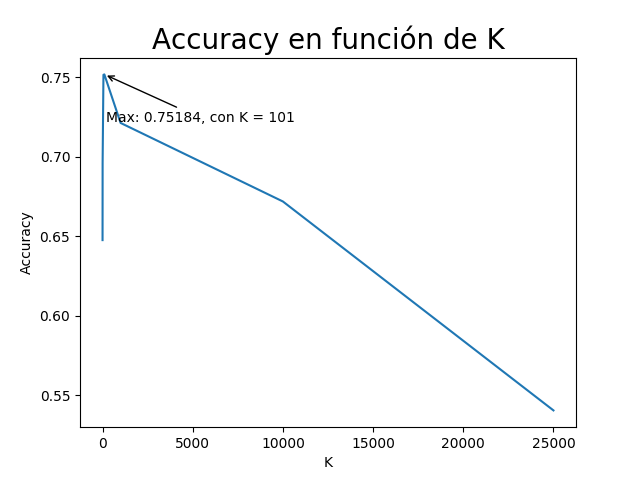
\includegraphics[ height=10cm, width=12cm]{../experimentos/graficos/graph_sin_pca_accuracy.png}
\caption{accuracy vs. valor de\textit{ k }sin PCA con F = 0.995 y f = 0.001}
\label{fig:exp_k}
\end{figure}

%conclusiones:
Luego de la experimentación, como se puede ver en la figura \ref{fig:exp_k}, verificamos nuestra hipótesis.
Observamos cómo las métricas ascienden positivamente para los primeros 101
valores de k, pero al tomar $k = 501$ las métricas comienzan a descender.

Podemos concluir mediante los resultados obtenidos que los mejores 2 valores de
k a considerar son $k = 51$ y $k = 101$, en donde 51 y 101 representan
respectivamente el 0,204\% y 0,404\% del total de valores de \textit{training}.\\

No nos quedamos conformes con el tiempo de ejecución de estas pruebas. Correr kNN para 6 valores distintos de\textit{ k }tardó aproximadamente 28 horas. Como queremos correr mucha más experimentación sobre distintas variables del programa queremos buscar una solución para poder acortar los tiempos. Lo que primero queremos ver es cómo cambian los resultados de la experimentación filtrando el vocabulario de palabras con otros valores que hagan los tiempos de ejecución más rápidos. Si no encontramos ningún filtro que cumpla con estas condiciones, vamos achicar el dataset de test ordenándolo de manera aleatoria antes.

Corrimos de vuelta el programa con los mismos parámetros cambiando solo los valores de \textbf{F}$ = 0.99$ y \textbf{f}$ = 0.01$.

\begin{figure}[H]
\centering
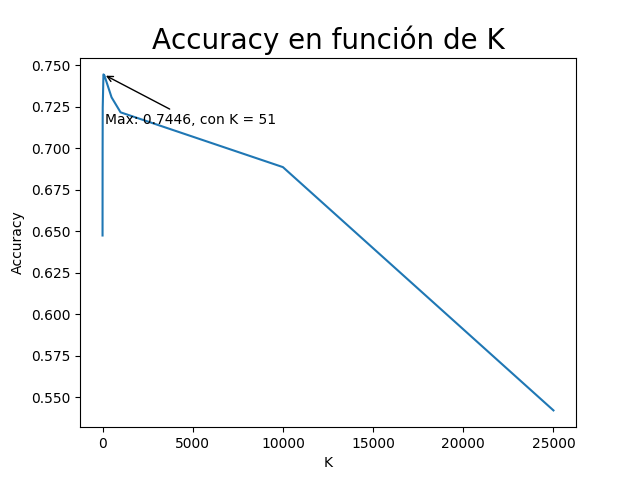
\includegraphics[ height=10cm, width=12cm]{../experimentos/graficos/graph_sin_pca_accuracy_FREQ_ORIGINAL.png}
\caption{accuracy vs. valor de\textit{ k }sin PCA con F = 0.99 y f = 0.01}
\label{fig:exp_k_orig}
\end{figure}
Con estos valores de filtrado la experimentación tardó aproximadamente 3 horas que significa un 90\% menos de tiempo que la prueba anterior.

Como podemos ver en la figura \ref{fig:exp_k_orig}, los mejores valores de\textit{ k }siguen siendo $k = 51$ y $k = 101$. El \textit{acurracy}, con estos valores de k, cambiando solo la frecuencia mínima y máxima de filtrado, varía en 0.007. Por lo tanto para las siguientes pruebas, salvo la de la sección \ref{sec:knnfrec}, vamos a filtrar el dataset con \textbf{F}$ = 0.99$ y \textbf{f}$ = 0.01$.

\subsubsection{Experimentación sobre frecuencia de palabras}
\label{sec:knnfrec}
%hipotesis
A continuación nos propusimos probar cómo varía la métrica de \textit{accuracy} al cambiar
la cantidad de palabras frecuentes y poco frecuentes que eliminamos de
nuestros \textit{Bag of Words}.
Recordamos que llamamos \textbf{f} a la frecuencia de palabras mínima a partir de la cual guardamos
palabras y \textbf{F} la frecuencia máxima a partir de la cual borramos palabras.

Suponemos que al tener una menor cantidad de palabras para cada reseña el
\textit{accuracy} al correr kNN va a ser más alto y al tener mayor cantidad de palabras va a ser peor.
Esto es debido a que las palabras más y menos frecuentes suelen meter más ruido
de lo que ayudan a clasificar.

%pruebas y gráficos
Para las pruebas, elegimos 3 valores de \textbf{f} y 3 de \textbf{F} y probamos cada valor de \textbf{f} con cada valor de \textbf{F}.
Corrimos las pruebas con $k = 51$, ya que en el experimento anterior vimos que
es un\textit{ k }razonable en cuanto a calidad de resultados.

\begin{figure}[H]
\centering
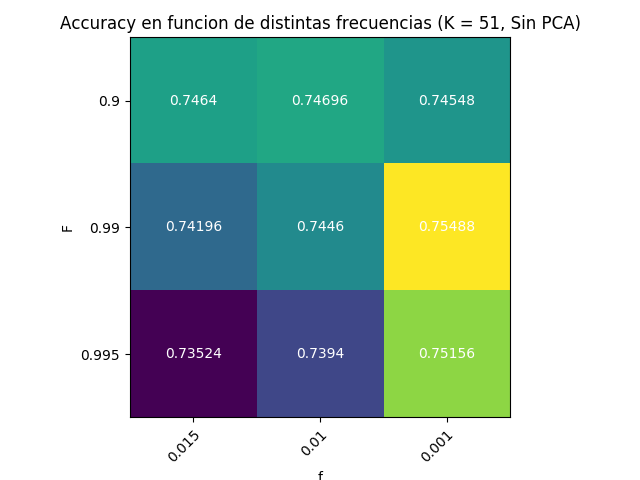
\includegraphics[ height=10cm, width=12cm]{../experimentos/graficos/graph_freq_accuracy51.png}
\caption{Accuracy vs. frecuencias con\textit{ k }= 51}
\label{fig:freq_k51}
\end{figure}

Al ver que nuestra hipótesis no se cumplió en la figura \ref{fig:freq_k51}, decidimos probar también con $k = 101$.

\begin{figure}[H]
\centering
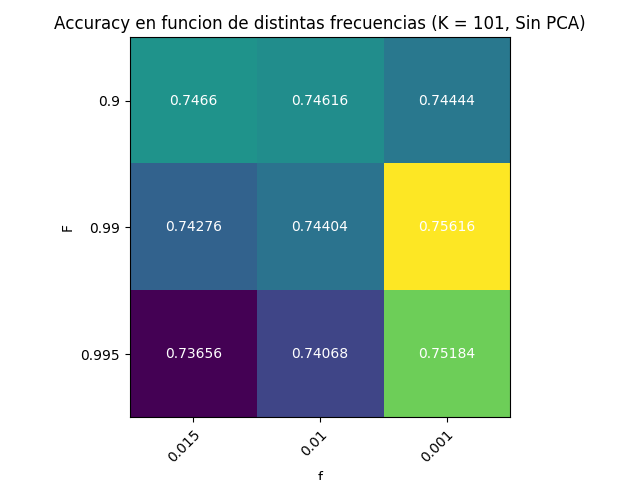
\includegraphics[ height=10cm, width=12cm]{../experimentos/graficos/graph_freq_accuracy101.png}
\caption{accuracy vs. frecuencias con\textit{ k }= 101}
\label{fig:freq_101}
\end{figure}

%conclusiones:
Tuvimos resultados parecidos para ambos\textit{ k }como se puede ver en la figura  \ref{fig:freq_k51} y \ref{fig:freq_101}, aunque ninguno concuerda con nuestra hipótesis inicial.

La combinación que menos accuracy tiene es nuestro \textbf{f} y \textbf{F} más altos, es decir,
la que elimina menos palabras de las más frecuentes (principalmente artículos
y palabras por el estilo) y muchas palabras poco frecuentes (palabras extrañas,
con \textit{typos} o en otros idiomas distintos al mayoritario, que es el inglés).

Por otro lado, la combinación que resultó en mayor \textit{accuracy}
fue cuando probamos el menor \textbf{f} y el \textbf{F} de tamaño medio.
Es decir, tenemos más \textit{accuracy} cuando borramos la menor cantidad de palabras poco
frecuentes y cuando borramos más palabras frecuentes que en el peor caso.

Esto nos dice que hay palabras que son poco frecuentes pero igualmente son
relevantes a la hora de clasificar, como pueden ser palabras que se usan en contextos
muy concretos pero con una tendencia positiva o negativa marcada.
Además, vemos que hay palabras con frecuencia alta que son relevantes, pero
hasta cierto punto. El equilibrio entre borrar pocas o muchas palabras
frecuentes parece ser cercano a $F = 0.99$.

\subsubsection{Experimentación con distintos tamaños del training dataset}
\label{sec:knnvstrain}
%hipotesis (Analizar tiempos y accuracy)

Otro experimento que nos parece interesante es cambiar el tamaño del dataset de entrenamiento.
Correremos el programa sin PCA usando el mismo dataset proporcionado por la cátedra, pero con la
diferencia que la cantidad de entradas de tipo training será un número variable y la cantidad
de entradas de tipo test serán los sobrantes. Para dividir esto, antes que nada, vamos a randomizar el dataset y
luego vamos a buscar igual cantidad de reseñas positivas que negativas para el dataset de training.

Sostenemos la hipótesis de que al aumentar el tamaño del dataset de training subirá el \textit{accuracy} de
nuestras predicciones. Pensamos esto debido a que al aplicar el algoritmo de kNN con tantos elementos
para comparar, suponemos que el vector correspondiente a una review negativa (o análogamente positiva)
tendrá muchos vecinos negativos. De la misma forma, si hay pocos elementos de training, esperamos que
una review negativa tenga pocos vecinos negativos, por lo tanto dando a lugar a vecinos positivos que
influyen en el rating.

Además, esperamos que eventualmente el crecimiento del \textit{accuracy} se estanque. Es decir, que en cierto
tamaño de dataset de training, deje de aumentar el \textit{accuracy} de las predicciones, debido a la cantidad de
vecinos de un elemento empieza a ser redundante para un \textit{k} razonable.

El siguiente gráfico muestra los resultados de correr predicciones sin PCA con diversos tamaños del training data,
con los \textit{ks} que mejores resultados dieron en experimentos anteriores. (51, 101, 501 y 1001)

%pruebas y gráficos

\begin{figure}[H]
\centering
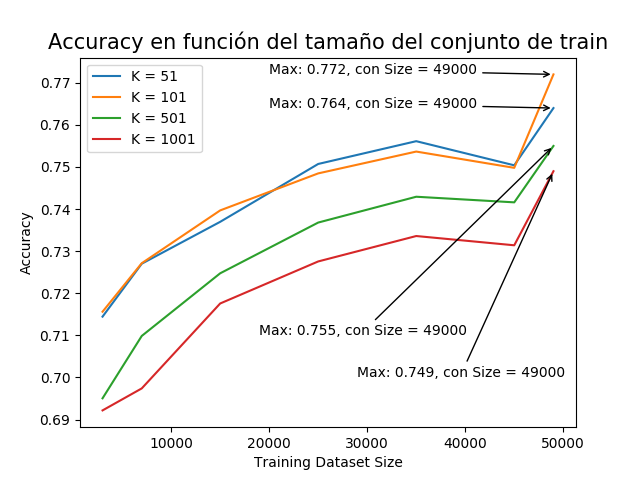
\includegraphics[ height=10cm, width=12cm]{../experimentos/graficos/graph_train_size_accuracy.png}
\caption{accuracy con distintos tamaños de training dataset}
\label{fig:exp_knn_train}
\end{figure}

Tal como esperabamos la figura \ref{fig:exp_knn_train} muestra que a medida que incrementa el tamaño del dataset de entrenamiento, también aumenta el
\textit{accuracy}. Se puede ver que cuanto mayor sea \textit{k}, los resultados de accuracy empeoran. Esto tiene sentido, dado que si hay más elementos en el algoritmo, da
lugar a nuevos vecinos para una predicción en particular que sólo son abarcables por un \textit{k} mayor.

No se puede observar que haya \textit{overfitting} al aumentar el tamaño del dataset de training, es decir, se observa que el \textit{acurracy} sigue aumentando al incrementar la cantidad de datos de entrenamiento.\\

Este experimento nos hizo pensar, que si bien aumentar el tamaño del conjunto de entrenamiento puede
mejorar las predicciones, también puede aumentar el tiempo de ejecución. Por lo tanto, planteamos un nuevo
experimento en donde ejecutamos 20 veces el algoritmo con $\textit{k} = 51$ fijo, para cinco tamaños distintos del conjunto de
entrenamiento (15000, 25000, 35000, 45000 y 49000) y luego medimos el tiempo de las predicciones
(es decir, sin tomar en cuenta el tiempo que toma cargar los datos y tokenizar).
En la figura \ref{fig:time_knn_train}, se puede ver el tiempo promedio de una \'unica predicci\'on.

\begin{figure}[H]
\centering
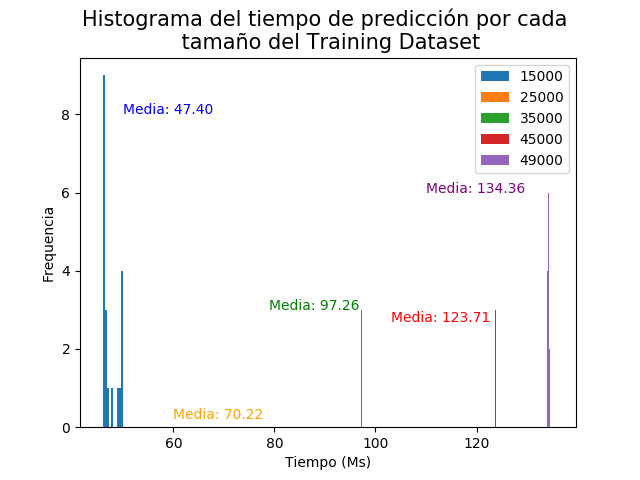
\includegraphics[ height=10cm, width=12cm]{../experimentos/graficos/graph_knn_vs_train_time.png}
\caption{tiempo de ejecución promedio de una predicción, con distintos tamaños de training dataset}
\label{fig:time_knn_train}
\end{figure}

%conclusiones:

Como era de esperar se ve que, en la figura \ref{fig:time_knn_train}, aumentar el tamaño del dataset de training implica más elementos contra quien comparar
distancias vectoriales en el algoritmo kNN, por lo tanto tiene sentido que aumente el tiempo de ejecuci\'on.
Esto es algo que tener en cuenta en la práctica, dado que se podría perder \textit{accuracy}, con tal de lograr
una predicci\'on mucho más veloz.

\subsection{Experimetación sobre PCA}

\subsubsection{Experimetación sobre tamaño del alpha}
%hipotesis
A continuación experimentamos sobre el valor de $\alpha$, siendo $\alpha$
la cantidad de componentes principales a considerar en el algoritmo de PCA.

Como hipótesis sostenemos que para los primeros valores de $\alpha$ el valor
de la métrica \textit{accuracy} va ir aumentando significativamente debido
a que las primeras componentes principales describen la mayor parte de la varianza de los datos.

Luego, a partir de determinado valor de $\alpha$ lo suficientemente grande,
conjeturamos que el valor de \textit{accuracy} comenzará a disminuir ya que
estaríamos considerando valores de la muestra de menor varianza y esto no
aportaría información sino que generaría ruido afectando la predicción de polaridad del vector.

%pruebas y gráficos
Experimentamos con distintos valores de $\alpha$, con $k = 1, 51, 101, 501, 1001, 24999$, y terminando el método de la potencia luego de 20 iteraciones.

\begin{figure}[H]
\centering
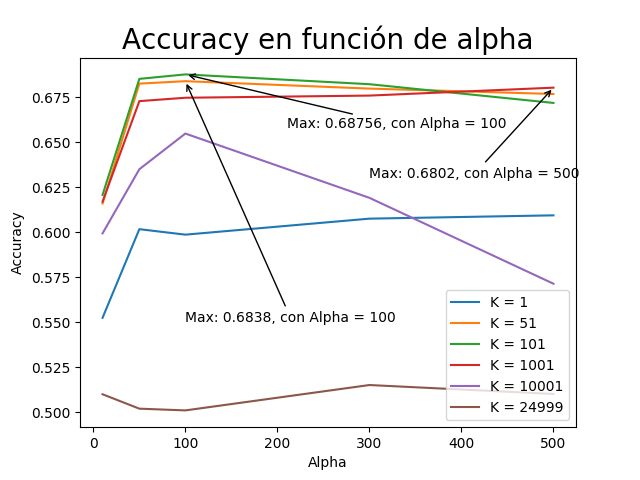
\includegraphics[ height=10cm, width=12cm]{../experimentos/graficos/graph_pca_accuracy.png}
\caption{accuracy vs. valor de alpha}
\label{fig:exp_alpha}
\end{figure}

%conclusiones:
Concluimos luego de la experimentación, viendo la figura \ref{fig:exp_alpha}, que el algoritmo de PCA es
particularmente útil para reducir la dimensionalidad de un grupo de datos.
Observamos que para valores bajos de $\alpha$ la accuracy aumenta debido a que
las primeras componentes principales describen la mayor parte de la varianza
de los datos (más, cuanto más correlacionadas estuvieran las variables originales).
Estos componentes de bajo orden a veces contienen el aspecto ``más importante''
 de la información, y las demás componentes se pueden ignorar.

\subsubsection{Experimentación sobre cantidad de iteraciones del Método de la Potencia}
%hipotesis
En esta sección mostraremos la experimentación realizada sobre distintos
valores de número de iteraciones antes de detener el Método de la Potencia
(En experimentos anteriores de PCA, este n\'umero era 20).
El mismo, como ya contamos anteriormente, es usado para calcular los autovectores
necesarios para PCA, por lo que resulta relevante detener el método en una
cantidad de iteraciones suficiente como para que el método converja, pero
no demasiado alto, ya que aumenta el tiempo de cómputo.

Nuestra hipótesis es que el \textit{accuracy} aumentará a medida que aumente
la cantidad de iteraciones, primero con una gran pendiente, pero luego de forma
más moderada hasta llegar a un techo.
Justificamos esto en que luego de cierta cantidad de iteraciones,
el método converge lo suficiente y no puede mejorar más de lo que la memoria
finita de los puntos flotantes se lo permite.

%pruebas y gráficos
A continuación, mostramos la experimentación realizada con $k = 51$ y $k = 101$,
y $\alpha = 100$ (el cual resultó ser de los mejores en el experimento anterior):

\begin{figure}[H]
\centering
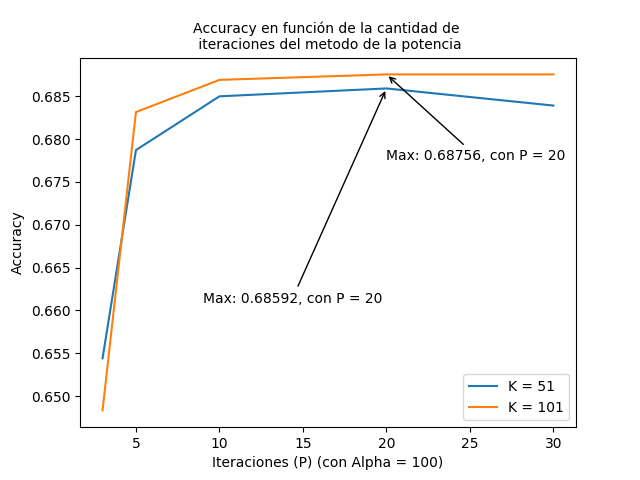
\includegraphics[ height=10cm, width=12cm]{../experimentos/graficos/graph_power_accuracy.png}
\caption{accuracy vs. cantidad de iteraciones del método de la potencia}
\label{fig:exp_met_potencia}
\end{figure}

%conclusiones:
Podemos observar que los resultados de la figura \ref{fig:exp_met_potencia} son los esperados.
En las pruebas con menor número de iteraciones se ve como el método mejora,
hasta que llega a 10 y comienza a aplanarse, sin demasiada diferencia
en la calidad de los resultados con un número de iteraciones superior.

\subsubsection{Experimentación sobre tamaño de training data}
%hipotesis (Analizar tiempos y accuracy)
Realizaremos distintas pruebas sobre el tamaño del dataset,
descripto anteriormente en la sección de Desarrollo, que utilizaremos como
Training Data para nuestro algoritmo. Este experimento es similar a uno
realizado anteriormente, pero ahora lo realizaremos con PCA.

Para este experimento, luego de randomizar el dataset proporcionado por la c\'atedra,
vamos a buscar igual cantidad de reseñas positivas que negativas para distintos tamaños
del dataset de training.

Lo que esperamos observar es, al igual que en el experimento anterior sin PCA,
que a medida que aumentemos el tamaño del Training Data, eligiendolo de igual manera que en la sección 3.1.3, el algoritmo prediga
cada vez mejor, resultando esto en un aumento en el valor de \textit{accuracy}.
Sin embargo, consideramos que este valor vaya creciendo cada vez más lento
a medida que el tamaño del Training Data es suficientemente grande,
debido a que ya no hay mucho más para ``aprender'', es decir, que la información
comienza a ser redundante y no aporta nuevo ``conocimiento'' de manera significativa.

Además, cuanto más grande sea el dataset de entrenamiento, hay que calcular
más distancias para realizar una predicción, por lo que esperamos que cada una
tome mayor tiempo.

%pruebas y gráficos
En los experimentos, utilizamos 5 tamaños distintos, que son los que vimos como más
relevantes en el experimento análogo a este sin PCA,
con $k = 51$, $k = 101$, $k = 501$ Y $k = 1001$. Al método de la potencia, lo terminamos luego de 20 iteraciones.

\begin{figure}[H]
\centering
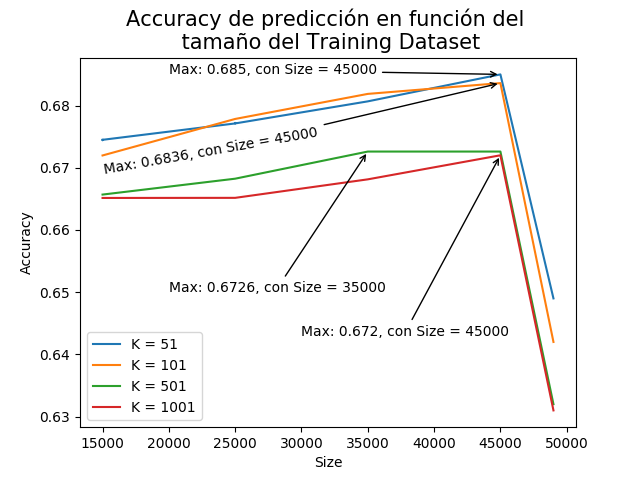
\includegraphics[ height=10cm, width=12cm]{../experimentos/graficos/graph_pca_vs_train_accuracy}
\caption{Acurracy de PCA con distintos tamaños de training dataset}
\label{fig:exp_pca_train}
\end{figure}

Para medir tiempos, ejecutamos las predicciones 20 veces, tomando el tiempo
de clasificar con kNN una vez que ya se redujeron las dimensiones con PCA.

\begin{figure}[H]
\centering
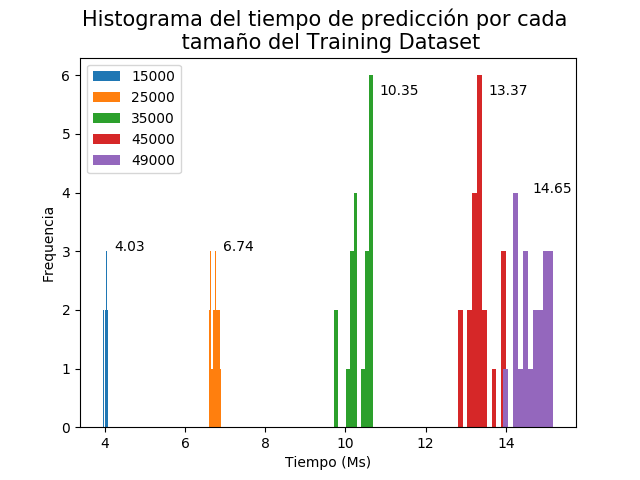
\includegraphics[ height=10cm, width=12cm]{../experimentos/graficos/graph_pca_vs_train_time.png}
\caption{tiempo de ejecución promedio de una predicción, con distintos tamaños de training dataset}
\label{fig:exp_pca_train_time}
\end{figure}

%conclusiones:
Posterior a la experimentación, viendo la figura \ref{fig:exp_pca_train}, podemos verificar nuestra hipótesis ya que el
valor de \textit{accuracy} aumenta a medida que aumentamos el tamaño del
Training Dataset, pero de forma gradual hasta que llega un punto donde el \textit{acurracy} empieza a descender. Esto nos indica que se produce \textit{overfitting}, es decir, llega un punto donde el dataset es tan grande que sobreentrenamos el sistema para poder predecir reseñas muy específicas que tienen poco relación con las reseñas que se testean.
Comparando con la Figura \ref{fig:exp_knn_train}, podemos ver que
el salto entre el \textit{accuracy} con el dataset de 15000 y el de 25000
es más pronunciado al usar kNN sin PCA que al agregarlo. Esto puede resultar de
que, al usar PCA, perdemos información que puede ser valiosa, incluyendo lo que
ganamos al aumentar el tamaño del Training Dataset.

Nuevamente, repitiendo los resultados del test sin PCA, observamos que hay un
\textit{trade-off}: con menos datos de entrenamiento,
las estimaciones resultan menos exactas, pero toman menos tiempo. De todos modos
al usar PCA el \textit{accuracy} creció relativamente poco con respecto a lo que
crecieron los tiempos de ejecución, como se ve en la figura \ref{fig:exp_pca_train_time}, por lo que es más factible usar un
dataset ``pequeño'' como el de 15000.

\subsection{Experimetación sobre kNN y PCA}
%hipotesis (Analizar tiempos y accuracy)
Para finalizar, nuestro último experimento consistirá en comparar el
tiempo de computo al ejecutar kNN con y sin PCA previo.
Nuestra hipótesis es que con PCA corra más rápido que sin, dado que disminuye
el tamaño de los vectores.

%pruebas y gráficos
Utilizamos los valores $k = 51$ y $\alpha = 100$, que en experimentos
anteriores han mostrado ser de los mejores. Computamos 18 veces los resultados,
midiendo los tiempos exclusivamente de kNN (es decir, sin contar el tiempo
de cargar los datos, tokenizar, o reducir dimensiones con PCA
en los casos que aplique).

\begin{figure}[H]
\centering
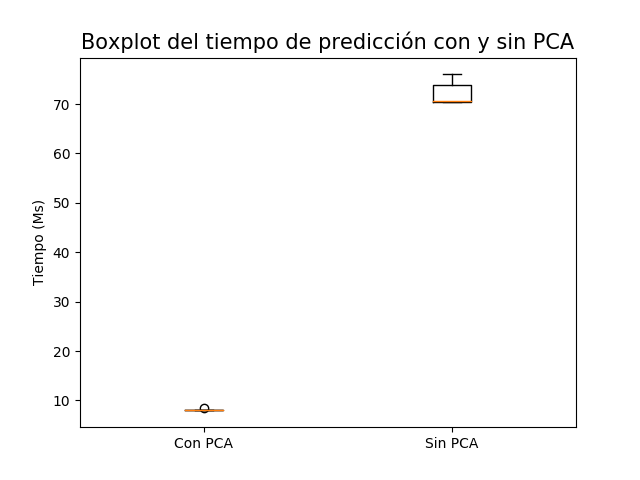
\includegraphics[ height=10cm, width=12cm]{../experimentos/graficos/graph_knn_vs_pca_time.png}
\caption{tiempo de ejecución promedio de una predicción, con y sin PCA previo}
\label{fig:exp_pca_knn}
\end{figure}

%conclusiones:
Como esperábamos, se ve en la figura \ref{fig:exp_pca_knn} que, los tiempos de ejecución bajan al ejecutar PCA antes de hacer
kNN. La contraparte es que, como se puede ver en las figuras ~\ref{fig:exp_k}
y ~\ref{fig:exp_alpha}, el \textit{accuracy} con PCA no supera el 70\%,
mientras que sin PCA llega a superar el 74\%.
La experimentación realizada nos hace pensar que, al usar PCA,
nos encontramos con un \textit{trade-off} entre velocidad y exactitud de resultados.
Esto puede resultar del hecho de que PCA descarta información
que puede resultar valiosa para la clasificación.
También es posible que la data no contenga ruido suficiente como para que
utilizar PCA mejore las métricas.
Resulta de interés realizar una experimentación más exhaustiva para comprobar que efectivamente
no existan hiperparámetros que consigan que utilizar PCA aumente el \textit{accuracy},
aunque queda fuera del alcance del presente trabajo.
% Esto nos muestra que, al usar
% PCA, nos encontramos con un \textit{trade-off} entre velocidad y exactitud
% de resultados. Esto puede resultar del hecho de que PCA descarta información
% que puede resultar valiosa para la clasificación.

\section{Conclusiones}
%Esta secci´on debe contener las conclusiones generales del trabajo. Se deben mencionar
%las relaciones de la discusi´on sobre las que se tiene certeza, junto con comentarios
%y observaciones generales aplicables a todo el proceso. Mencionar tambi´en posibles
%extensiones a los m´etodos, experimentos que hayan quedado pendientes, etc.

En este trabajo realizamos un análisis del funcionamiento de kNN y PCA para un
caso muy particular (análisis de polaridad de comentarios de películas), pero
de gran interés para poder realizar en el futuro un análisis social o de mercado,
además de por su posible uso en otros tipos de textos.

Con los distintos experimentos que realizamos, pudimos ver que estos
métodos tiene el potencial de predecir sentimientos con una exactitud
de hasta el 75\% aproximadamente, que no es para nada despreciable.

Sin embargo, estos resultados los conseguimos al utilizar kNN \textbf{sin PCA}.
Como vimos en la sección anterior, usar PCA nos presenta un \textit{trade-off}
entre velocidad y exactitud.

Algo interesante visto en la experimentación fue la relación entre las palabras
filtradas por frecuencia y la calidad de los resultados.
En estos, contrario a nuestras expectativas previas, pudimos ver que hay
palabras poco frecuentes que resultan realmente relevantes.
Consideramos que un posible estudio a realizar en el futuro podría venir por
el lado de ver qué palabras concretas son, para tener una mejor comprensión
de lo que sucede, y probar con una mayor variedad de porcentajes para filtrar palabras.

Finalizando este trabajo, concluimos que kNN es un método simple pero efectivo
para clasificar, al menos en el contexto particular de este trabajo, y que
PCA es una buena herramienta para acompañar a kNN cuando necesitamos acelerar
el mismo, y podemos permitirnos una reducción en la exactitud del análisis.

\section{Referencias}
% TODO: usar https://en.wikibooks.org/wiki/LaTeX/Bibliography_Management
\begin{thebibliography}{9}
\bibitem{BO}
Bo Pang, Lillian Lee, et al. Opinion mining and sentiment analysis. Foundations and Trends in Information Retrieval, 2(1-2):1-135, 2008.

\bibitem{LIU}
Liu, B. (2007). Web Data Mining. Exploring Hyperlinks, Contents, and Usage Data. Alemania: Springer. p. 412.

\bibitem{Weiss}
Weiss, S. (2005). Text Mining. Predictive Methods for Analyzing Unstructured information. (en inglés). EUA: Springer. p. 6.

\bibitem{IMDB}
Internet Movie DataBase, https://www.imdb.com/

\bibitem{pot}
R. L. Burden y J.D.Faires, Numerical Analysis, Ninth Edition. p. 576 (9.3 The Power Method)

\bibitem{Maas}
Andrew L. Maas, Raymond E. Daly, Peter T. Pham, Dan Huang, Andrew Y. Ng, and
Christopher Potts. Learning word vectors for sentiment analysis. In Proceedings of the
49th Annual Meeting of the Association for Computational Linguistics: Human Language
Technologies, pages 142–150, Portland, Oregon, USA, June 2011. Association for Compu-
tational Linguistics.

\end{thebibliography}

\appendix
%En el ap´endice A se incluir´a el enunciado del TP. En el ap´endice B se incluir´an los
%c´odigos fuente de las funciones relevantes desde el punto de vista num´erico. Resultados
%que valga la pena mencionar en el trabajo pero que sean demasiado espec´ıficos para
%aparecer en el cuerpo principal del trabajo podr´an mencionarse en sucesivos ap´endices
%rotulados con las letras mayusculas del alfabeto romano. Por ejemplo: la demostraci´on
%de una propiedad que aplican para optimizar el algoritmo que programaron para resolver
%un problema.

\section{Enunciado}
\label{ap:enunciado}
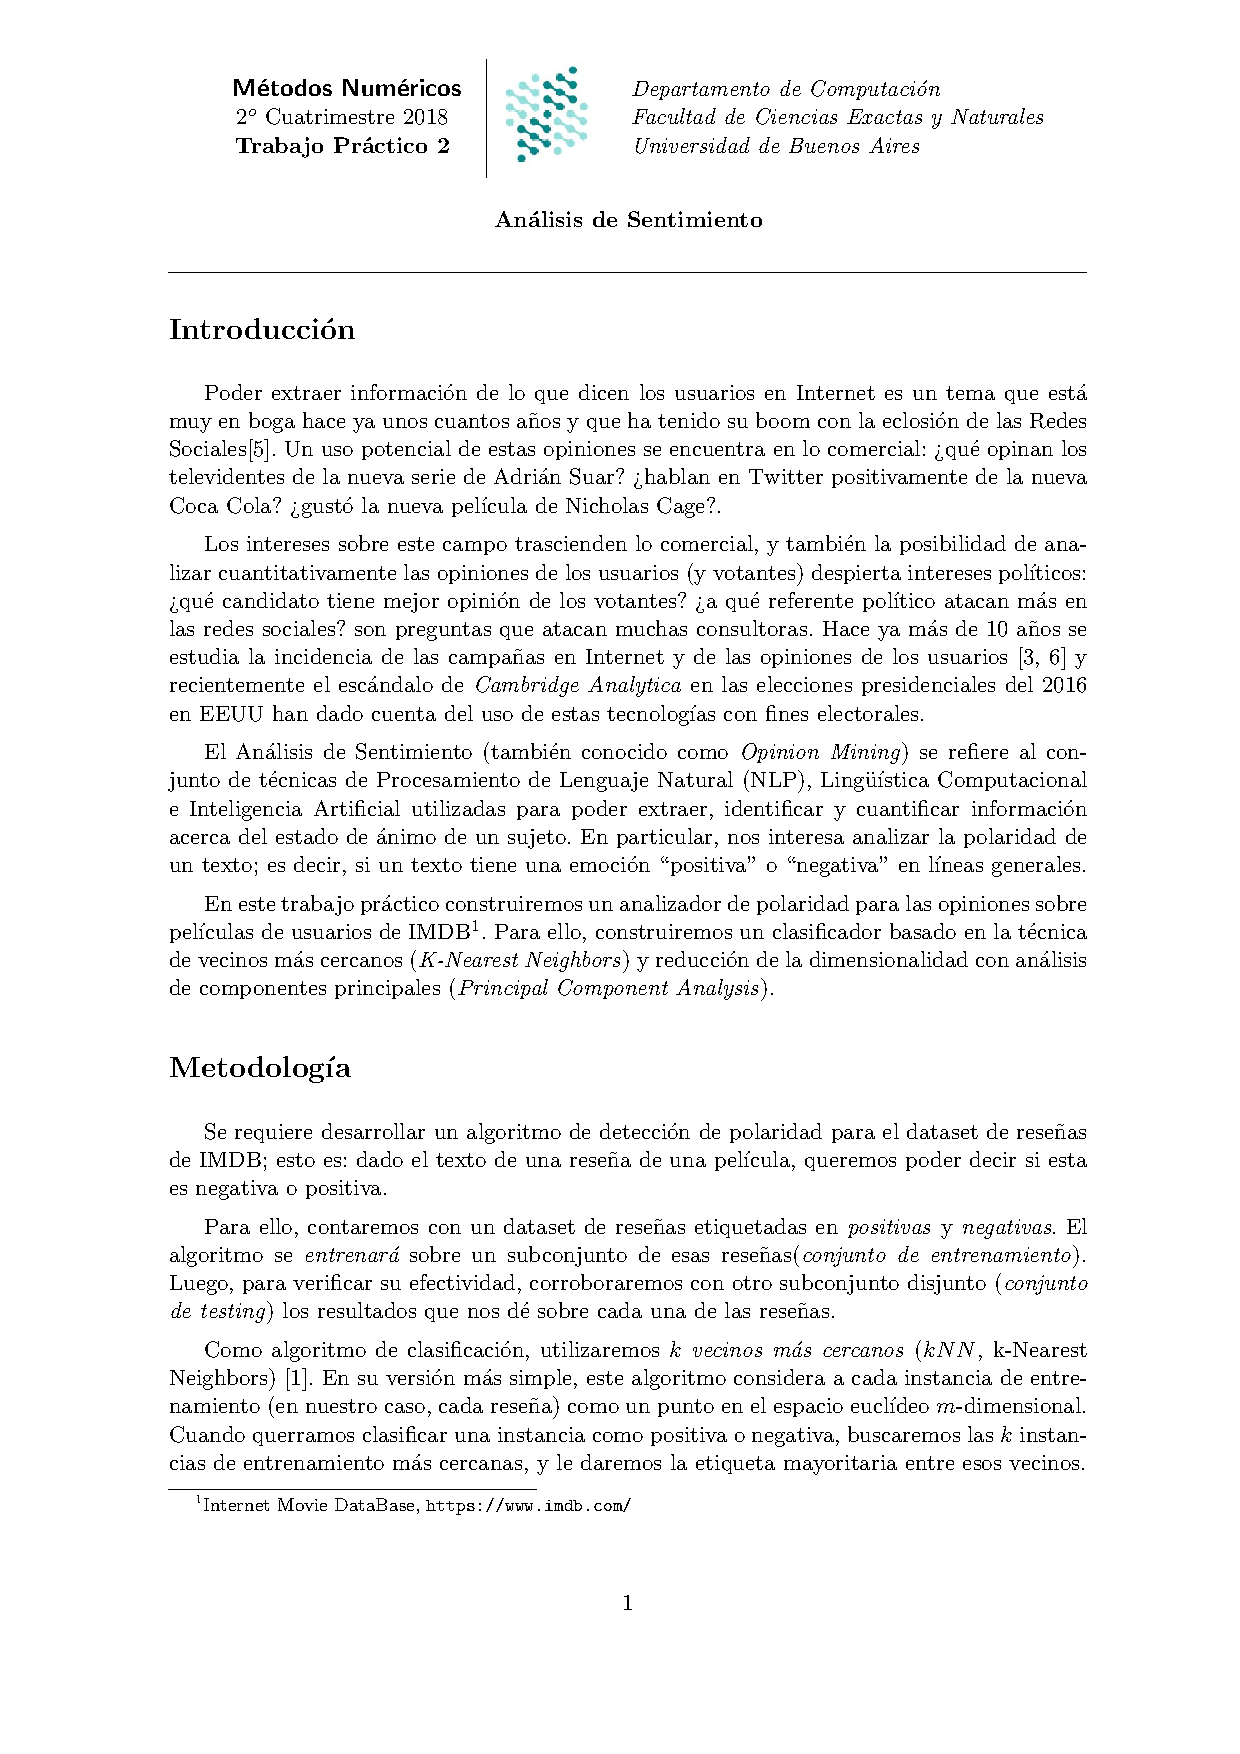
\includepdf[pages=-]{../docs/tp2.pdf}

\section{Código fuente relevante numéricamente}

Código de búsqueda de k vecinos más cercanos (kNN):
\begin{lstlisting}
// Utiliza dist, que simplemente calcula la distancia Manhattan dados dos vectores
bool knn(const VectorizedEntriesMap &entries, const std::vector<double> &words, int k) {
    std::vector<std::pair<double, bool> > distancias;

    for (auto entry:entries) {
        distancias.push_back({
            dist(words, entry.second.bag_of_words),
            entry.second.is_positive});
    }

    MinHeap heapDistancias(distancias.begin(), distancias.end());

    int cant_pos = 0;
    for (int i = 0; i < k; i++) {
        std::pair<double, bool> vecino = heapDistancias.top();
        heapDistancias.pop();

        if (vecino.second) {
            cant_pos++;
        }
    }

    return cant_pos >= (k - cant_pos);
}
\end{lstlisting}

Código de PCA:
\begin{lstlisting}
// Este codigo es parte del metodo pca, escrito en pca.cpp
// Solo ponemos este segmento ya que es el realmente relevante numericamente
// El resto es preparacion de datos y manejo de datos precalculados

// Vector para calcular autovector
std::vector<double> v(dimReviews);
// Autovectores calculados
std::vector<std::vector<double>> autovectores;
for (unsigned int i = 0; i < alpha; i++) {
    std::cerr << "                           " << "\r";
    std::cerr << "Buscando autovector " << i << "\r";
    double autovalor = metodoPotencia(covarianza, v, p);
    autovectores.push_back(v);
    reducirAutovalores(covarianza, v,
                       autovalor);
}
salidas = autovectores;
\end{lstlisting}

Código de reducirAutovalores, que dado una matriz y un autovalor de la misma,
cambia la matriz de forma que ese autovalor cambie por 0:
\begin{lstlisting}
void reducirAutovalores(
    std::vector<std::vector<double>> &B,
    std::vector<double> &v,
    double autovalor) {
    for (unsigned int i = 0; i < B.size(); i++) {
        for (unsigned int j = 0; j < B.size(); j++) {
            B[i][j] -= autovalor * v[i] * v[j];
        }
    }
}
\end{lstlisting}
\pagebreak
Código del Método de la Potencia:
\begin{lstlisting}
double metodoPotencia(
    const std::vector<std::vector<double>> &A,
    std::vector<double> &v,
    int numeroIteraciones) {
    obtenerVectorRandom(v);

    for (int iteracion = 0; iteracion < numeroIteraciones; iteracion++) {
        v = normalizar(A * v);
    }
    return (v * (A * v)) / (v * v);
}
\end{lstlisting}

\end{document}
